%\documentclass[a4paper]{article}
\usepackage[utf8]{inputenc}
\usepackage[spanish, es-tabla, es-noshorthands]{babel}
\usepackage[table,xcdraw]{xcolor}
\usepackage[a4paper, footnotesep=1.25cm, headheight=1.25cm, top=2.54cm, left=2.54cm, bottom=2.54cm, right=2.54cm]{geometry}
%\geometry{showframe}

%\usepackage{wrapfig}			%Wrap figure in text
\usepackage[export]{adjustbox}	%Move images
\usepackage{changepage}			%Move tables

\usepackage{tikz}
\usepackage{amsmath}
\usepackage{amsfonts}
\usepackage{amssymb}
\usepackage{float}
\usepackage{graphicx}
\usepackage{caption}
\usepackage{subcaption}
\usepackage{multicol}
\usepackage{multirow}
\usepackage{wrapfig}
\setlength{\doublerulesep}{\arrayrulewidth}
\usepackage{booktabs}
\usepackage[numbib, nottoc, notlot, notlof]{tocbibind}

\usepackage{hyperref}
\hypersetup{
    colorlinks=true,
    linkcolor=blue,
    filecolor=magenta,      
    urlcolor=blue,
    citecolor=blue,    
}

%Change Font Size

% #1 = size, #2 = text
\newcommand{\setparagraphsize}[2]{{\fontsize{#1}{6}\selectfont#2 \par}}		%Cambia el size de todo el parrafo
\newcommand{\setlinesize}[2]{{\fontsize{#1}{6}\selectfont#2}}				%Cambia el font de una oración

\newcommand{\note}[1]{
	\begin{center}
		\huge{ \textcolor{red}{#1} }
	\end{center}
}

%FONTS (IMPORTANTE): Compilar en XeLaTex o LuaLaTeX
\usepackage{anyfontsize}	%Font size
\usepackage{fontspec}		%Font type

\usepackage{etoolbox}
\usepackage{todonotes}

\newcommand{\observacion}[2]{  \ifnumequal{1}{#1}{ { \todo[inline,backgroundcolor=red!25,bordercolor=red!100]{\textbf{Observación: #2}} } }{  }  }

\setcounter{topnumber}{2}
\setcounter{bottomnumber}{2}
\setcounter{totalnumber}{4}
\renewcommand{\topfraction}{0.85}
\renewcommand{\bottomfraction}{0.85}
\renewcommand{\textfraction}{0.15}
\renewcommand{\floatpagefraction}{0.8}
\renewcommand{\textfraction}{0.1}
\setlength{\floatsep}{5pt plus 2pt minus 2pt}
\setlength{\textfloatsep}{5pt plus 2pt minus 2pt}
\setlength{\intextsep}{5pt plus 2pt minus 2pt}

\newcommand{\quotes}[1]{``#1''}
\usepackage{array}
\newcolumntype{C}[1]{>{\centering\let\newline\\\arraybackslash\hspace{0pt}}m{#1}}
\usepackage[american]{circuitikz}
\usetikzlibrary{calc}
\usepackage{fancyhdr}
\usepackage{units} 

\graphicspath{{../Control de posición no lineal/}{../Control de fuerza no lineal/}{../Control híbrido no lineal/}{../Referencias/}{../Deducción de modelo/}{../Conclusiones/}}

\pagestyle{fancy}
\fancyhf{}
\lhead{22.99 - Automación Industrial}
\rhead{Lambertucci, Londero B., Maselli, Mechoulam}
\rfoot{Página \thepage}

%Items con bullets y no cuadrados
\renewcommand{\labelitemi}{\textbullet }


%\begin{document}

\subsection{Caracterización del problema}
Se desarrolla un control cartesiano no lineal para el manipulador RR. Además se debe considerar una zona prohibida, representada por todo aquel valor por encima de una pared, descrita en el plano XY pro la siguiente ecuación:
\begin{equation}
y=2-x
\end{equation}

Se busca que el manipulador se desplace desde el punto (1;-1;0) al (1;1;0). Para generar la trayectoria se utiliza la función \textbf{jtraj} del toolbox de matlab de Peter Corke.

\subsection{Esquema de control}
El modelo de control propuesto es el conocido como linealización por realimentación. Es fundamental para este tipo de control tener un gran conocimiento de la planta, ya que básicamente se realiza el control como si fuese lineal, con un esquema tipo PD, con la diferencia que se agrega a la acción de control la respuesta no lineal de la planta.
%gracias al conocimiento del modelo no lineal de la planta y sus variables de estado.

\begin{figure}[H]
	\centering
	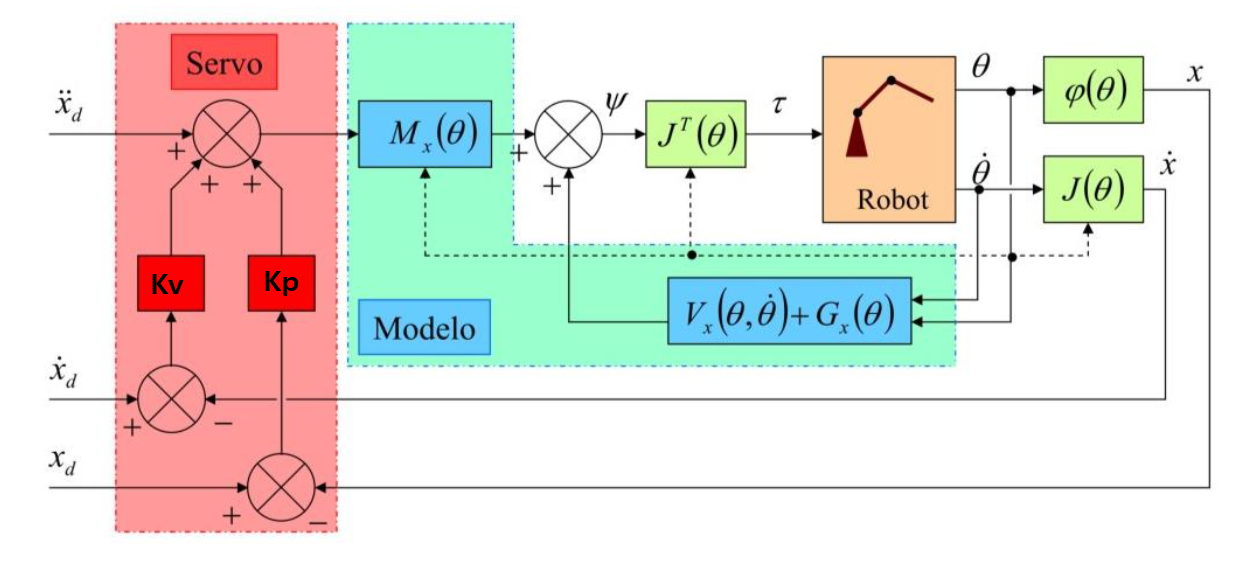
\includegraphics[width=0.8\linewidth]{ImagenesControl de posición no lineal/modelo_control_p}
	\caption{Topología del control de posición cartesiano no lineal.}	
	\label{fig:control_p_modelo}
\end{figure}

Cabe mencionar que las matrices $M_x,\ V_x, \ y \ G_x$ se encuentran en espacio cartesiano. La manera de pasar de las mismas en espacio joint es la siguiente:
\begin{equation*}
M_x(\Theta) = J^{-T}(\Theta) M(\Theta) J^{-1}(\Theta)
\end{equation*} 
\begin{equation*}
V_x(\Theta , \dot{\Theta}) = J^{-T}(\Theta) \left( V(\Theta , \dot{\Theta}) - M(\Theta) J^{-1}(\Theta) \dot{J}(\Theta) \dot{\Theta} \right)
\end{equation*} 
\begin{equation*}
G_x(\Theta) = J^{-T}(\Theta) G(\Theta) 
\end{equation*}

\observacion{\verObs}{HABLAR DE VALORES DE GANANCIAS}

Para obtener las ganancias del sistema se empleo el método de Ziegler-Nichols. De esta forma, los valores obtenidos fueron:
\begin{itemize}
	\item Kv = [80 0;0 80].
	\item Kp = [250 0; 0 250].
\end{itemize}

\subsection{Resultados}
Se realizó el sistema en simulink. Se obtuvieron los siguientes gráficos.
En estos se pueden observar los ángulos de los manipuladores en espacio de joint.

Como el primer rotacional hace una trayectoria de $-\frac{\pi}{2}$ hacia $0$, y el segundo, si bien el punto inicial y final son el mismo, se desvía con el propósito de seguir la trayectoria cartesiana indicada.

\begin{figure}[H]
	\centering
	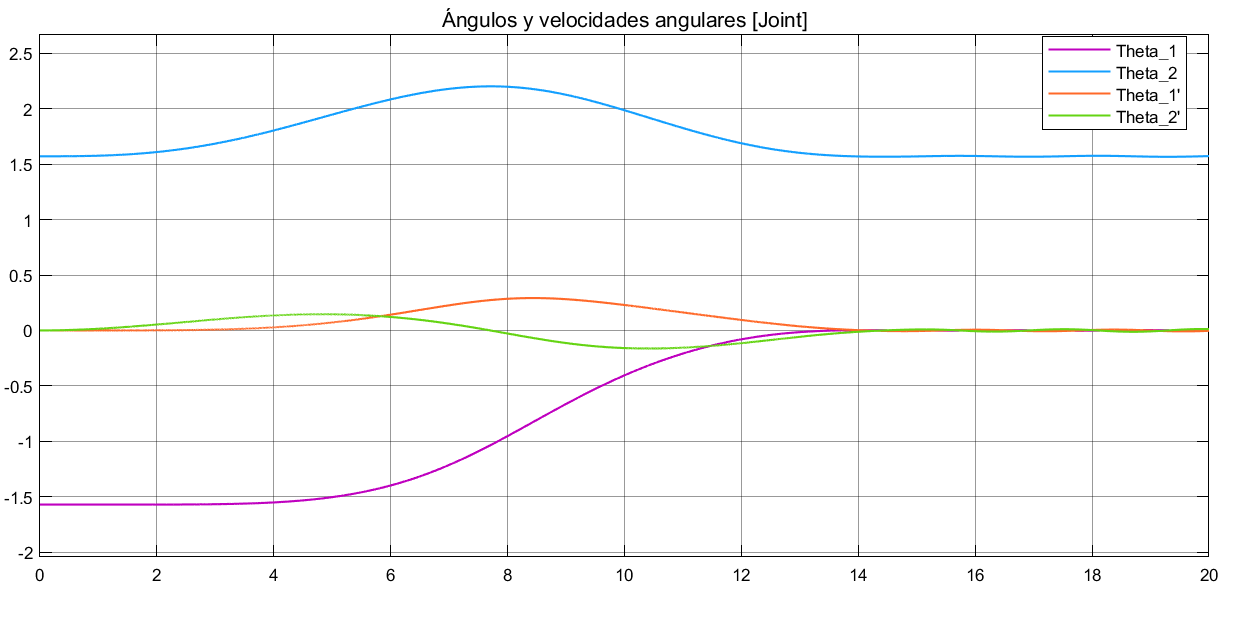
\includegraphics[width=0.8\linewidth]{ImagenesControl de posición no lineal/1_3_a}
	\caption{Ángulos en función del tiempo en espacio joint.}	
	\label{fig:athetas}
\end{figure}


En la Figura (\ref{fig:apos}) se ven tanto las referencias como las coordenadas reales que tomó el EE, con un error porcentual menor del 20$\%$ en el eje X y menor del 5$\%$ en el eje Y. 

\observacion{\verObs}{Porcentaje desconocido.}

\begin{figure}[H]
	\centering
	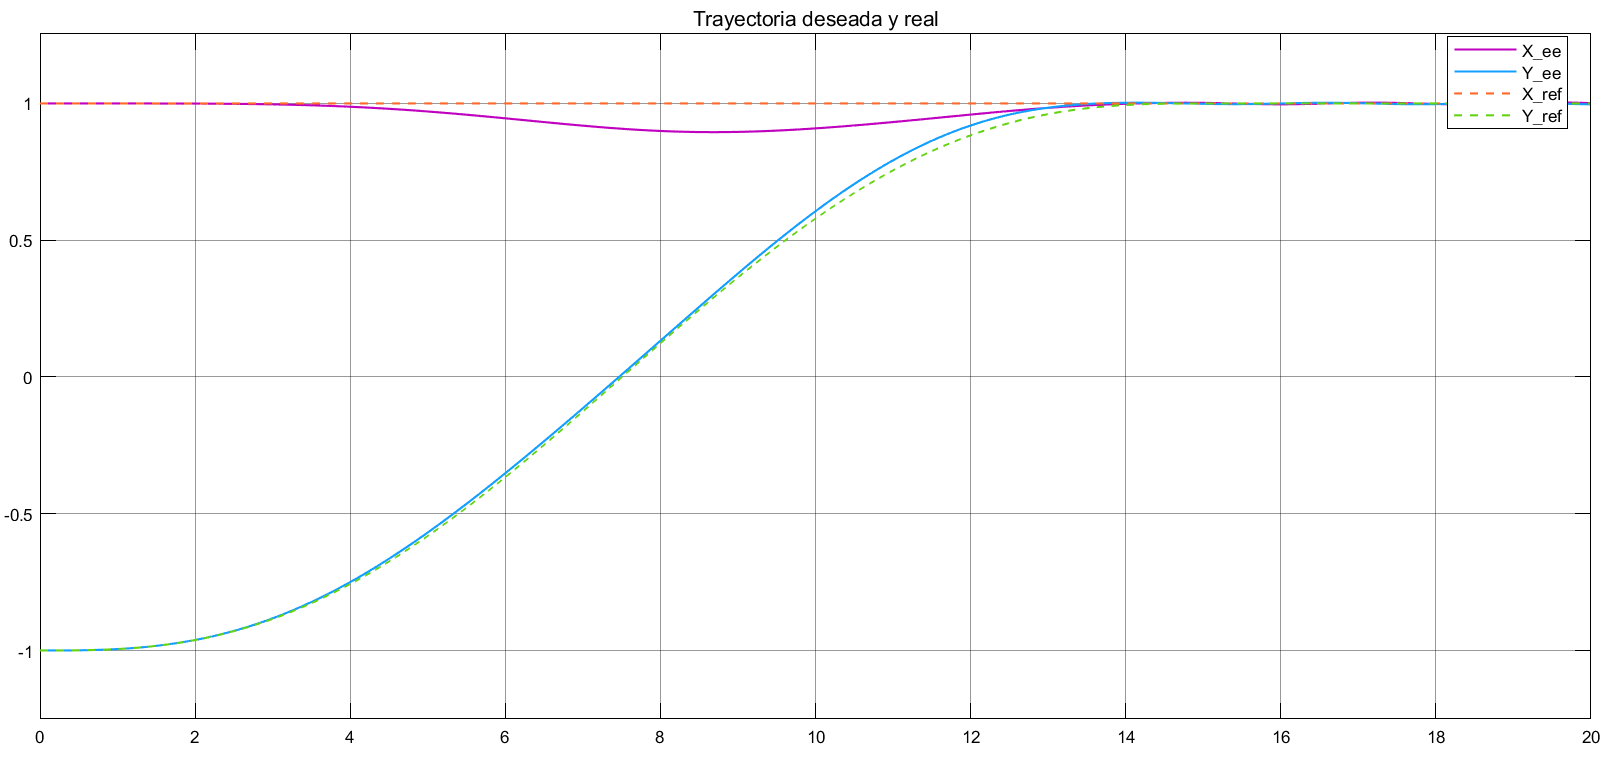
\includegraphics[width=0.8\linewidth]{ImagenesControl de posición no lineal/1_3_b}
	\caption{Posición deseada y real del EE.}	
	\label{fig:apos}
\end{figure}
La trayectoria descripta por el EE se observa claramente en la siguiente imagen.
\begin{figure}[H]
	\centering
	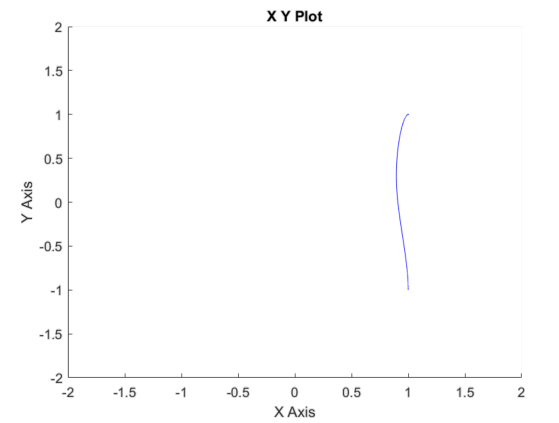
\includegraphics[width=0.5\linewidth]{ImagenesControl de posición no lineal/1_3_c}
	\caption{Gráfico XY.}	
	\label{fig:axy}
\end{figure}

Ademas se le incluyó un disturbio a la planta tanto en posición como en velocidad. Este disturbio sucede en el segundo 14. Se observa en los siguientes gráficos como el manipulador es afectado por el mismo y luego vuelve rápidamente a la referencia.

\begin{figure}[H]
	\centering
	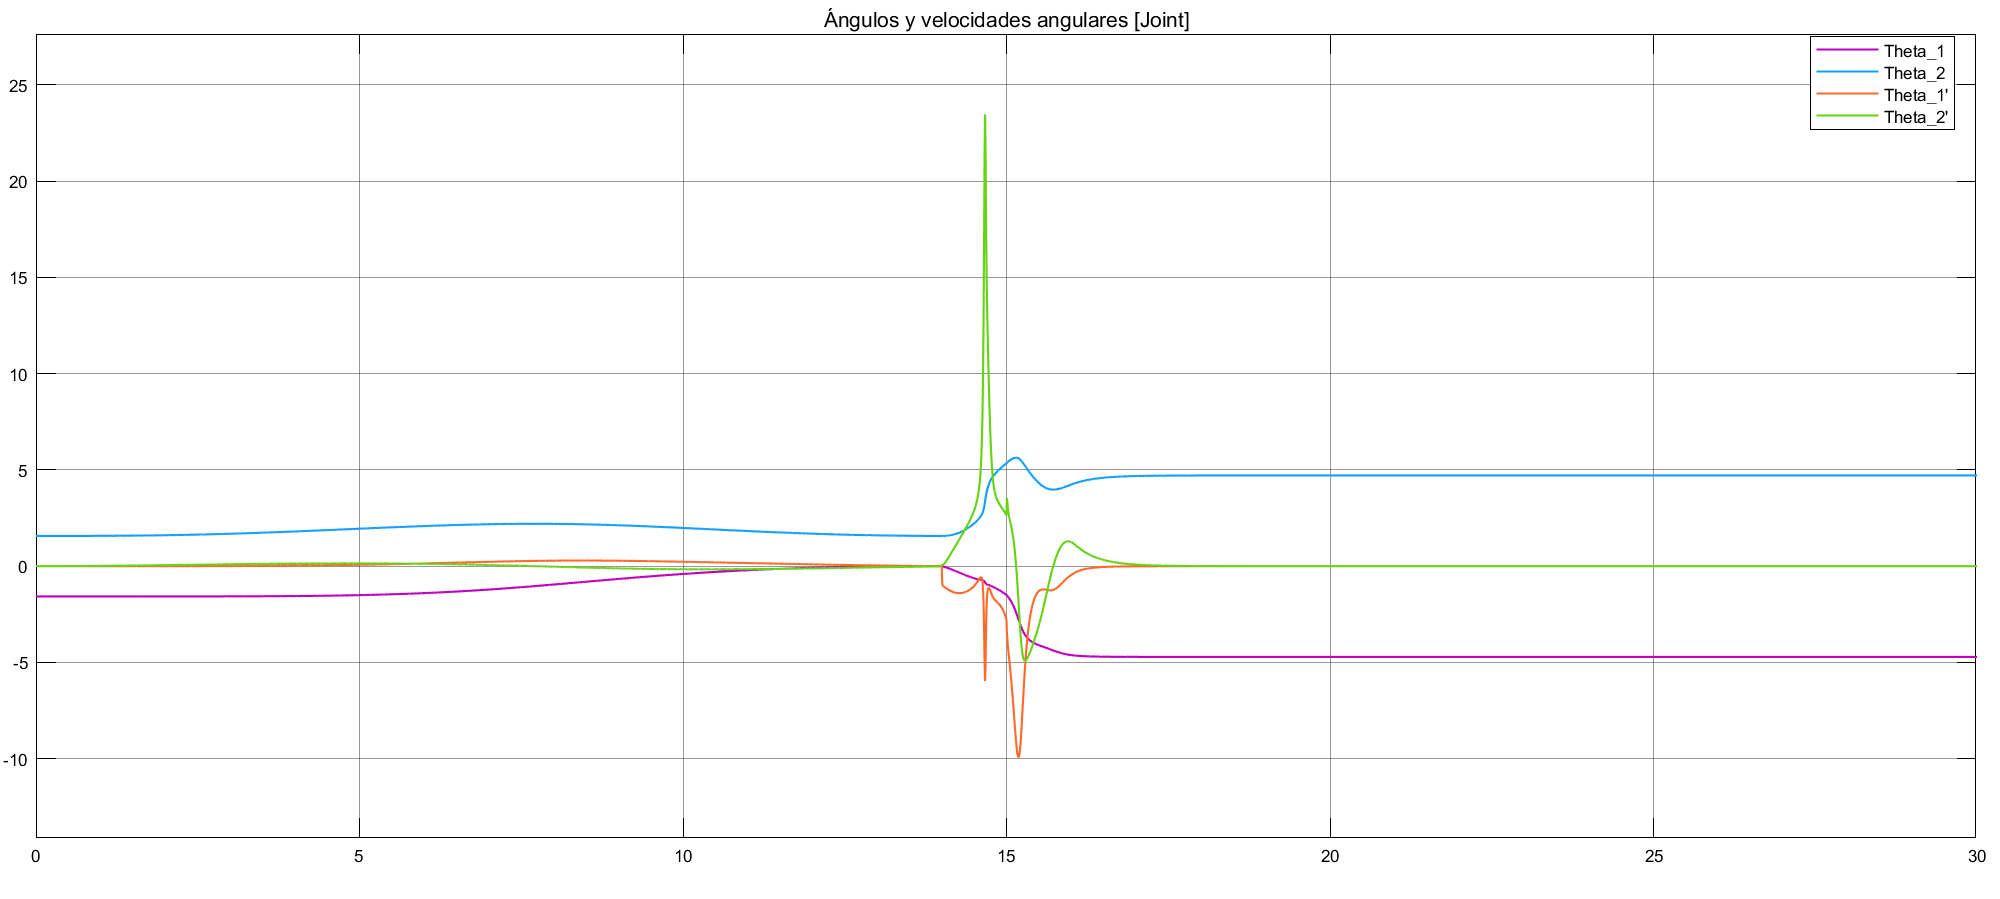
\includegraphics[width=0.8\linewidth]{ImagenesControl de posición no lineal/1_3_e_a}
	\caption{Ángulos en función del tiempo en espacio joint.}	
	\label{fig:athetasd}
\end{figure}

\begin{figure}[H]
	\centering
	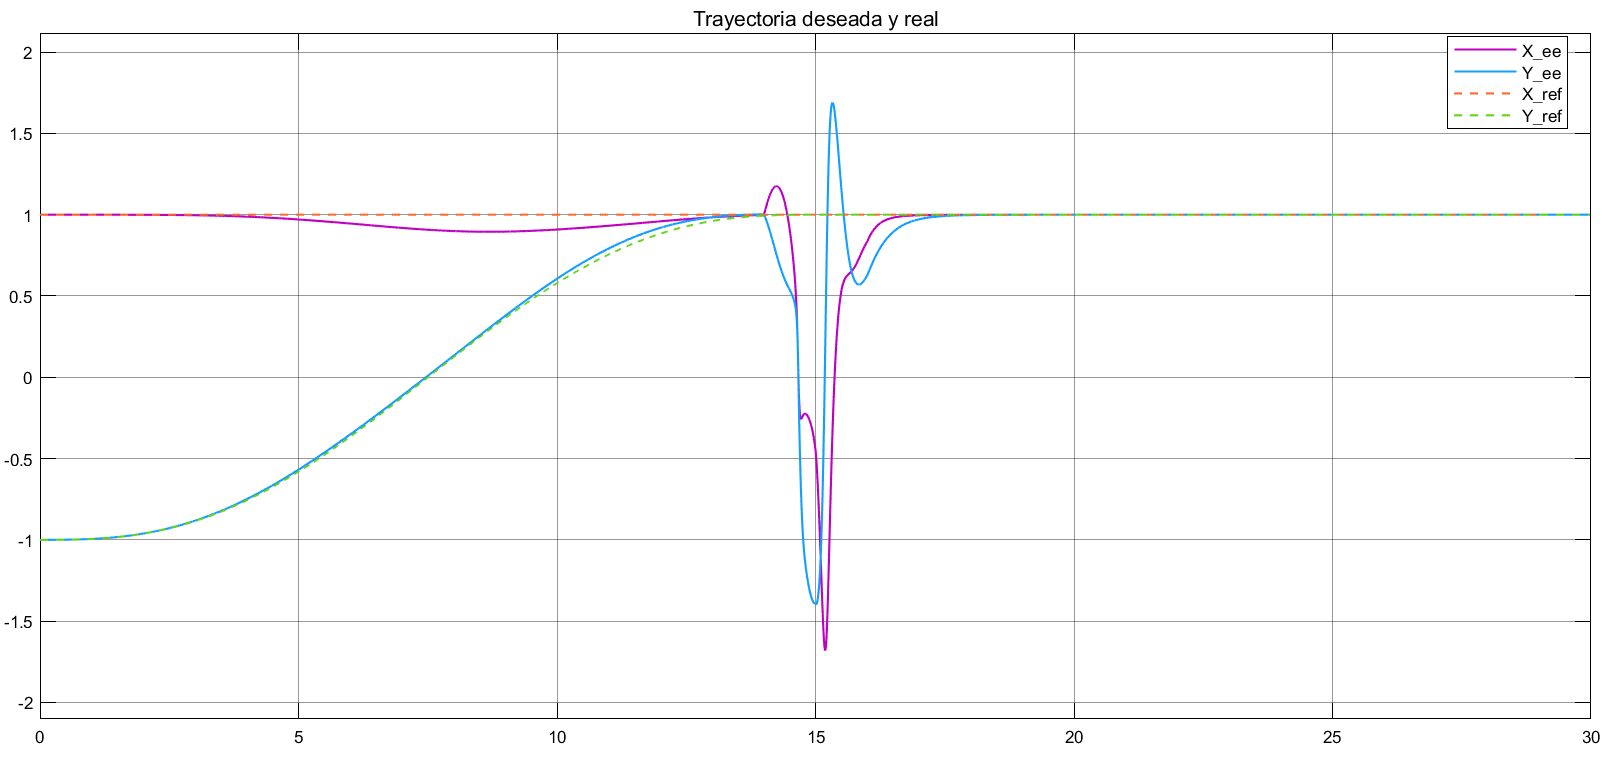
\includegraphics[width=0.8\linewidth]{ImagenesControl de posición no lineal/1_3_e_b}
	\caption{Posición deseada y real del EE.}	
	\label{fig:aposd}
\end{figure}

\begin{figure}[H]
	\centering
	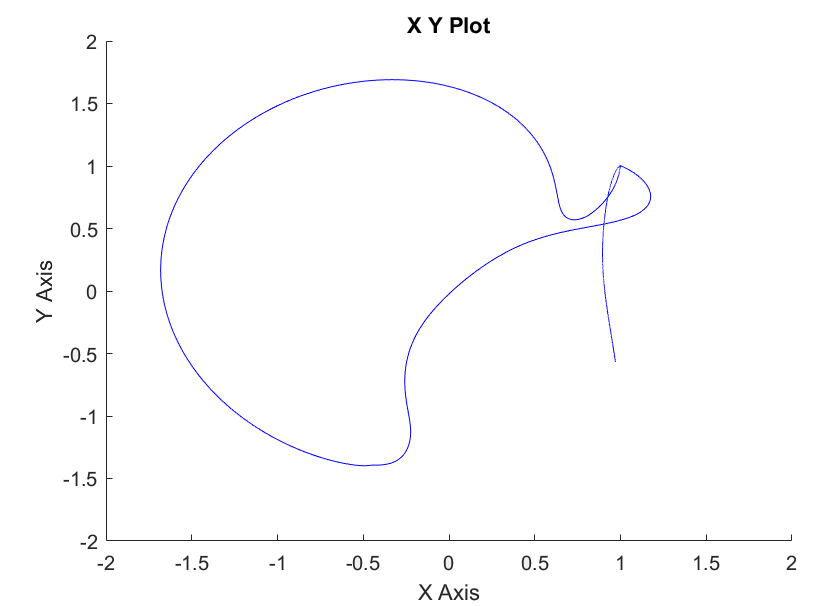
\includegraphics[width=0.5\linewidth]{ImagenesControl de posición no lineal/1_3_e_c}
	\caption{Gráfico XY.}	
	\label{fig:axyd}
\end{figure}

De manera similar al caso presentado en la Sección (\ref{sec:posic}), se utilizó el método de Ziegler-Nichols. De esta forma, los valores obtenidos fueron:
\begin{itemize}
	\item Kv = [150 0;0 150].
	\item Kp = [250 0; 0 250].
\end{itemize}

%\end{document}